\begin{mydef}
	Un carré est un quadrilatère qui possède \kw{quatre angles droits} et \kw{quatre côtés de même longueur}.
\end{mydef}

\begin{myprops}
	\textbf{Si} un quadrilatère est un carré \textbf{alors} 
	\begin{itemize}
		\item ses \kw{quatre cotés} ont la \kw{même longueur};
		\item il a \kw{quatre angles droits};
		\item ses \kw{diagonales} sont \kw{perpendiculaires} et ont la \kw{même longueur}.
	\end{itemize}
\end{myprops}

\begin{myex}
	\begin{center}
		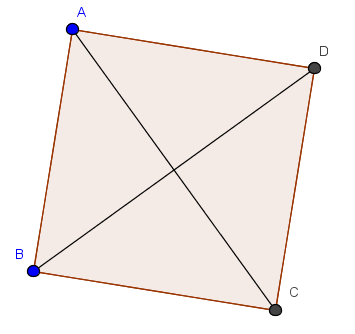
\includegraphics[scale=0.15]{carre}
	\end{center}

	ABCD est un carré donc \begin{itemize}
		\item $AB = BC = CD = DA$;
		\item  $\widehat{ABC} = \widehat{BCD} = \widehat{CDA} = \widehat{DAB} = 90\degree$;
		\item $AC = BD $;
		\item $(AC) \perp (BD)$.
	\end{itemize}
\end{myex}